%% LyX 2.0.5.1 created this file.  For more info, see http://www.lyx.org/.
%% Do not edit unless you really know what you are doing.
\documentclass[12pt,english]{report}
\usepackage{mathptmx}
\renewcommand{\familydefault}{\rmdefault}
\usepackage[T1]{fontenc}
\usepackage[latin9]{inputenc}
\usepackage[a4paper]{geometry}
\geometry{verbose,tmargin=2cm,bmargin=2cm,lmargin=2cm,rmargin=2cm,headheight=1cm,headsep=1cm,footskip=1cm}
\setcounter{secnumdepth}{2} % Changed from 3 to 2. 0-chapter 1-section 2-subsection 
\setcounter{tocdepth}{2} % Changed from 3 to 2. 0-chapter 1-section 2-subsection 
\setlength{\parskip}{\medskipamount}
\setlength{\parindent}{0pt}
\usepackage{verbatim}
\usepackage{pdfpages}
\usepackage{graphicx}
\usepackage{subfig} %% This package has to be here
\usepackage{setspace}
\usepackage{arabtex}
\usepackage[numbers]{natbib}
\usepackage{nomencl}


\begin{document}

\chapter{Letters Classifier}


{\color{blue}Online handwriting recognition is one of the very complex and challenging problems [1][2][3] because of variability on size, writing style of hand-printed characters , and duplicate pixels caused by a hesitation in writing or interpolate non-adjacent consecutive pixels caused by fast writing. \cite{verma2004feature}}

It is a classification of each unknown object into one of a finite set of categories or classes. 
\emph{
\begin{itemize}
\item state the general problem definition of classification. [3-4 sentences]
\item talk about pattern classification [2 sentences]
\item talk about the different types and approaches of letters classification [1 paragraph]
\end{itemize}
}

In the on-line Arabic text recognition, these categories could be a whole word, word-parts, letter or even strokes. The problem that makes the recognition of on-line handwriting recognition difficult is variation of shapes of the characters resulting from writing habits, styles, and the social and educational level of the writer.\\
 

In this chapter we will describe a fast letters classifier. As mentioned in the overview in chapter \ref{[]}, our goal is to perform strokes segmentation and letters recognition while the stroke is being written. Thus, the performance of the of the classification process is a critical part.  

This stage produces a list of candidate characters for an input sequence and the letter position this sequence. The  
      
Our classifier contains 4 distinct databases, one for each position. The figure below describes the process through until it reaches its final position in the corresponding database.

Each Recognition process contains two parts, the learning from samples system and the object classification system. .....\\
In section \ref{sec:letters_learning} we describe our Letters learning process and in \ref{sec:substrokes_classification} we describe our classifier. 

\section{Letters Learning}
\label{sec:letters_learning}

\emph{ TODO: show a diagram of the letters learning system}

\section{Sub-strokes Classification}
\label{sec:substrokes_classification}

\emph{ TODO: show a diagram of the letters learning system}

{\color{blue}
The process of online handwriting recognition can be broken down into a few general steps:
preprocessing,
feature extraction and
classification.
The purpose of preprocessing is to discard irrelevant information in the input data, that can negatively affect the recognition.[3] This concerns speed and accuracy. Preprocessing usually consists of binarization, normalization, sampling, smoothing and denoising.[4] The second step is feature extraction. Out of the two- or more-dimensional vector field received from the preprocessing algorithms, higher dimensional data is extracted. The purpose of this step is to highlight important information for the recognition model. This data may include information like pen pressure, velocity or the changes of writing direction. The last big step is classification. In this step various models are used to map the extracted features to different classes and thus identifying the characters or words the features represent. [http://en.wikipedia.org/wiki/Handwriting\_recognition]}



\newpage{}

\section{Samples Preprocessing}

The data obtained by the digitizer is composed of points in the plane that represent the trajectory scribed by the writing instrument on the tablet surface. Usually, samples are taken in time intervals, thus slow pen motion regions are oversampled and fast motion regions are under-sampled. In addition, when such devices are used to capture handwriting strokes, the shapes of the strokes present a jagged form and the obtained data is non-uniform and noisy. Further imperfections are caused by hand vibrations and duplicated sampled points resulted from hesitant writing. This noise should be reduced as much as possible since it influence the further processes, such as feature extraction and classification \cite{al2011online} \cite{huang2009preprocessing}.  
To overcome the flaws mentioned, preprocessing operations are usually applied. The preprocessing steps imposes certain uniform structure on the data to comply with the input structure required by the latter parts of the system, such that vector length, sequence bounds, etc.\\

\emph{TODO: mention other preprocessing approaches mentioned in the literature, like rotation normalization, slant normalization, and missing points interpolation. see \cite{jaeger2001online}.}

As seen in figure \ref{[]} and \ref{}, preprocessing is performed in both letters learning and classification of strokes.
Preprocessing is also done in the segmentation phase, however, not all steps mentioned in this section are performed. For more information see section \ref{[]}

Our preprocessing phase include three steps in the following order: \emph{Normalization and Translation}, \emph{Noise Elimination} and then \emph{Smoothing and Re-sampling}.\\ 

In figure \ref{fig:D_before_after_preprocessing} we show a sample of the letter \RL{d} sequence before and after preprocessing.\\ 

In the next sub-sections we will describe in details each part of the preprocessing procedure.

\begin{figure}
	\centering
        \subfloat[]{
            \label{fig:letter_before_preprocessing}
            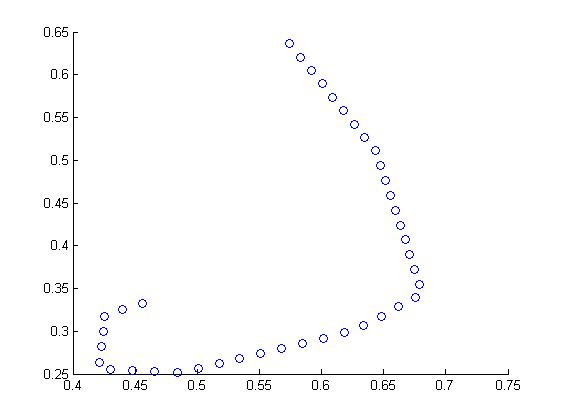
\includegraphics[width=0.5\textwidth]{./figures/letter_before_preprocessing}
        }
        \subfloat[]{
           \label{fig:letter_after_preprocessing}
           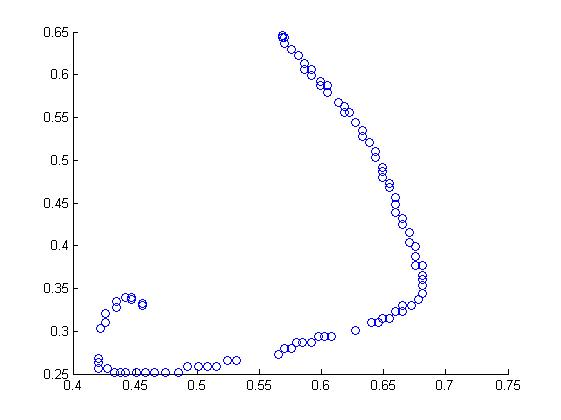
\includegraphics[width=0.5\textwidth]{./figures/letter_after_preprocessing}
        }        
    \caption{The letter \RL{d} before (a) and after (b) preprocessing}
   \label{fig:D_before_after_preprocessing}
\end{figure}

\emph{refer to the slant and Rorarion normalization, i.e. why we don't do it. Is slant common in Arabic?
}

\subsection{Normalization and Translation}

Size normalization is done to achieve a uniform size of the bounding box surrounding the pattern. This is done to enable the classifier to recognize the sequence pattern even when the stroke is written in different sizes. Shape similarity algorithms tend to be sensitive for non-uniform shapes size, thus this procedure is important and can be found in many approaches in the literature. 
However, this method could not be applied since normalization is done in our system on the stroke level which could contain a letter, at least.
In our approach size normalization was applied on each stroke such that all strokes have $[0,1]\times[0,1]$ bounding box but retain their original aspect ratio. We include in this step also translation of the sequence's center of gravity to the origin point $[0,0]$.
Given the stroke sequence $S=\{p_i\}_{i=1}^{n}$, the normalized sequence $\bar{S}=\{\bar{p_i}\}_{i=1}^{n}$ is calculated by: 

\begin{equation}
{\bar x_i} = {{\left( {{x_i} - {\mu _x}} \right)} \over W},{\bar y_i} = {{\left( {{y_i} - {\mu _y}} \right)} \over W}
\end{equation}
Where
\begin{equation}
\mu  = \left( {{\mu _x},{\mu _y}} \right) = \left( {{1 \over N}\sum\limits_{i = 1}^N {{x_i}} ,{1 \over N}\sum\limits_{i = 1}^N {{y_i}} } \right)
\end{equation}
\begin{equation}
W = \max \left( {{d_x},{d_y}} \right)
\end{equation}
\begin{equation}
{d_x} = {x_{\max }} - {x_{\min }};\,\,\,{d_y} = {y_{\max }} - {y_{\min }}
\end{equation}
\begin{equation}
{x_{\max }} = \mathop {\max }\limits_i \left( {{x_i}} \right),\,\,{x_{\min }} = \mathop {\min }\limits_i \left( {{x_i}} \right),\,\,{y_{\min }} = \mathop {\min }\limits_i \left( {{y_i}} \right),\,\,{y_{\min }} = \mathop {\min }\limits_i \left( {{y_i}} \right)
\end{equation}  

\subsection{Noise Elimination}
The input obtained by the digitizer may contain a large amount of noise which is mainly duplication of points. In this process redundant points are filtered out and a similar sequence with fewer points is obtained.
In order to eliminate redundant points irrelevant for pattern classification and screening out unwanted noise and vibrations in the letter inscription we have used the \emph{Douglas-Peucker Polyline Simplification algorithm} described in \cite{douglas1973algorithms}. Briefly, it is a line simplification algorithm to reduce the number of vertices in a piecewise linear curve according to a specified tolerance. The algorithm is also known as \emph{Iterative Endpoint Fit}. The resulted curve is a skeletonized angular sequence. The Normalization is done before the Simplification, since we need a constant simplification parameter $\varepsilon$ which was tuned for $1\times1$ bounds. 
Assuming the stroke presentation is a sequence of points $S$, the sensitivity parameter that was used in our work is:
\begin{equation}
\varepsilon  = {1 \over {200}}\sqrt {{d_x}^2 + {d_y}^2}
\end{equation}

\begin{figure}
\centering
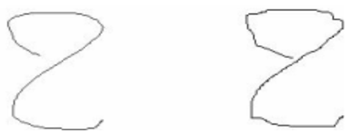
\includegraphics[width=0.7\textwidth]{./figures/ha_simplification}       
\caption{Non Simplified representation of the letter \RL{.h} (Ha) is shown on the right. A simplified version is shown on the left. \emph{TODO: change the pictures to something better}}
\label{fig:ha_simplification}
\end{figure}

\subsection{Smoothing and Re-sampling}
As a result of the simplification process the points are not distributed uniformly along the stroke trajectory. Naturally, there are less point in relatively straight areas and a higher amount of points in the curved areas of the stroke.\\ 
%if we wont use simplification we can write this: The re-sampling is needed to prevent the unbalanced sampling density, which may be influenced by the sampling rate and the user non-uniform letter drawing. 
The re-sampling produces equidistant smoothed data sequence. 
The Re-sampling is performed using splines interpolation as follows:\\
Given a stroke $S=\{p_i\}_{i=1}^{n}$ and the re-sampling target number $R$, let $\{X(a_i)\}_{i=1}^{n}$ and $\{Y(a_i)\}_{i=1}^{n}$ represent the x-axis and the y-axis sequences with respect to the parameter $a_i$ which is defined as follows:

\begin{equation}
a_i=a_{i-1}+arclen(p_{i-1},p_i) 
\end{equation}  

\begin{equation}
X(a_i)=x_i 
\end{equation}  

The arc-length of the stroke is given by $L=a_n$.\\

A piecewise linear interpolations $q_X(a)$ and $q_X(a)$ are created for the $X$ sequence and $Y$ sequence respectively.
The breaks are the $a_i$ sequence and the coefficient of the linear polynomial are $\alpha_{i} = \frac{X(a_i)-X(a_{i-1})}{a_{i}-a_{i-1}}$ 

\emph{[we use quadratic splines for smoothing and simplification.]}

let $t_i=i\frac{L}{R}$ for $i=0,...,R$.
The re-sampled sequence is given as follows:
\begin{equation}
\widehat{S}=\{(q_X(t_i),q_Y(t_i))\}_{i=1}^{R}
\end{equation}

The target number of points is set to 40. We had to find a number that is good enough for both long and short strokes since strokes can span over a single letter or a whole WP.

\emph{[TODO: show the following images: 1. the scattered stroke, 2. X and Y as a function of t., 3. X and Y resampledm and 3. the stroke resampled. ]}

\emph{[TODO: talk about splines.]}

\emph{TODO: talk about the other smoothing techniques as described in \cite{jaeger2001online} -- Online handwriting recognition: the NPen++ recognizer}


\begin{figure}
\centering
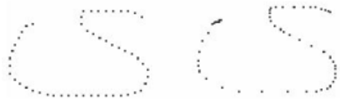
\includegraphics{./figures/y_resampling}       
\caption{Representation of a non-resamples sequence of the letter \RL{y} (Y) is shown in the right. The re-sampled version is shown on the left.}
\label{fig:y_resampling}
\end{figure}

\newpage{}

\section{Features Extraction}

Answer the following:
\begin{itemize}
\item Goal and importance
\item shape descriptor properties
\item types of features - local vs. global and simple vs. complex - examples, (hierarchical) 
\item Discussion - why did we decided to concentrate on shape context and MAD.
\item Discussion - Is combining several feature extraction technique is recommended?
\item Results - show the difference between MAD and SC.
\end{itemize}

Feature extraction is certainly one of the important parts of any pattern classification system. It aims is to cull informative parameters for learning and recognition of patterns.  Most classification methods require that patterns be represented in a fixed dimensional feature space that is often incompatible with input data. Poor feature extraction and selection will always result in a poor system performance, regardless of the ingeniousness of the learning and classification algorithms \cite{parizeau2001character}.\\

Feature extraction is commonly used in pattern recognition. While its goal is same in all fields, feature extraction methods operate differently in different domains. For instance, in the image retrieval field, the input data (i.e. the image) is too large and suspected to be redundant. In this case, feature extraction techniques are used to reduce the representation of the input data into a compact representation set of features. However, In the shape recognition domain, the input data is compact and feature extraction techniques are used to transform it into feature vectors, which are usually referred to as shape descriptors. Shape descriptors offer discriminative characterization to capture the perceptual dissimilarity between two shapes. Unlike in the first case, the raw quantity of data contained in feature vector usually exceeds the amount of data in the input data.\\

The goal of a shape descriptor is to be able to effectively find perceptually similar shapes from a database. Shape descriptors are usually in the form of vectors that are produced to represent a given shape feature and attempts to quantify perceptual similarities between shapes. That is to say, shapes which are found perceptually similar by human have resembling descriptor than from shapes that are different from the others. Effective shape descriptor must present some essential properties such as translation, rotation and scale invariance. It also must be as robust as possible against noise so that variously distorted shapes which are tolerated by human beings when comparing shapes. This is known as the robustness requirement.\cite{zhang2004review}\\

Low computation complexity is an important characteristic of a desirable shape descriptor. Efficiency of a descriptor is equally important as effectiveness due to the on-line retrieval demand. The descriptors should be represented and stored compactly. The size of a descriptor vector must not be too large. 

A shape descriptor is usually measured according to several principles which include good retrieval accuracy, compact features, low computation complexity and robust retrieval performance. \cite{kim2000region}

Many shape description have been developed in order to improve the segmentation and recognition rates. There are many different classifications and sub classifications of shape descriptors according to their method of operation.The most common classification is the classification for local and global descriptors. Local descriptors calculate some feature at each sample point. Simple local features include the y coordinate and tangent slope angle. \emph{Normalized curvature} and \emph{Ratio of tangent} \cite{hu1995invariant,hu1996hmm} are examples of more complex local shape descriptor. Descriptors such as cusps, crossings and loops are referred to as global descriptors and are calculated on the entire shape \cite{hu1997combining}.

For a detailed review on shape descriptors see \cite{zhang2004review} and \cite{yang2008survey}.

Many well known and powerful features operate on the contour of the shape. This is because many descriptors were developed for off-line handwriting recognition in which the shape is the script contour. In the on-line handwriting recognition, the input data is a sequence of points  and no contour is involved, however using features in on-line handwriting recognition that we originally developed for the off-line case is common. Saabne and El-Sanna have used shape context, a shape descriptor that was developed for contour based shapes, for the online handwriting recognition in \cite{saabni2009hierarchical}. Multi Scale shape context, a combination of three different shape contexts:
stroke, local neighborhood and global shape contexts, is used by Hu and Zanibbi in \cite{husegmenting} for on-line handwritten mathematical expressions segmentation.

In this work we have chosen to work with two shape descriptors, the Shape context descriptor and the tangent angle feature. The reason for this choice is that we wanted to investigate how both global and local features effectiveness in our proposed process. More information about these features are given in section \ref{sec:shape_context} and in section \ref{sec:mad}

In this work we have selected two features to work with, the Shape Context and the Multi Angular Descriptor. Generally, when considering shapes, the contour of the shape is taken into account, thus the following 2 shape descriptors is defined using the contour of the shape. However in the on-line writing recognition case, the features are applied upon the stroke sequence. 

\subsection{Shape Context}
\label{sec:shape_context}
Belongie and Malik have presented a point matching approach named Shape Context \cite{belongie2002shape}. The Shape context is a shape matching approach that intended to be a way of describing shapes that allows for measuring shape similarity and the recovering of point correspondences. This approach is based on the following descriptor: Pick $n$ points on the shape's contour, for each point ${p_i}$ on the shape, consider the $n - 1$ other points and calculate the coarse histogram of the relative coordinates. Equation \ref{eq:sc_bins} is defined to be the shape context of ${p_i}$.

\begin{equation}
{h_i}(k) = \# \{q \ne p_i:(q - p_i) \in bin(k) \}
\label{eq:sc_bins}
\end{equation}

The bins are normally taken to be uniform log-polar space making the descriptor more sensitive to positions of nearby sample points than to those of points farther away. This distribution over relative positions is robust and compact, yet highly discriminative descriptor. The basic Idea of the Shape Context Descriptor is illustrated in Figure \ref{fig:shape_context_demo}. This can be calculated in $O(N^3)$ time using the Hungarian method. 

\begin{figure}
\centering
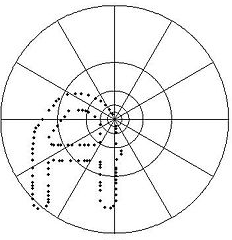
\includegraphics{./figures/shape_context_offline}       
\caption{Diagram of the log-polar bins used to compute the shape context.}
\label{fig:shape_context_demo}
\end{figure}

\begin{figure}
\centering
\subfloat[]{
    \label{fig:shape_context_offline}
    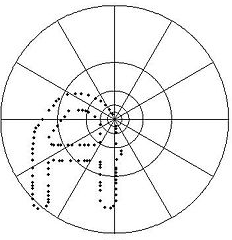
\includegraphics[width=0.5\textwidth]{./figures/shape_context_offline}
}
\subfloat[]{
	\label{fig:shape_context_online}
     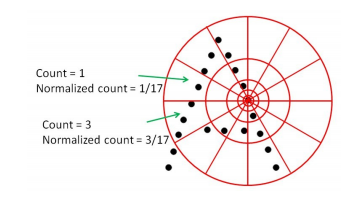
\includegraphics[width=0.5\textwidth]{./figures/shape_context_online}
}        
\caption{Diagram of the log-polar bins used to compute the shape context. On-line and off-line}
\label{fig:shape_context_demo}
\end{figure}

\subsection{Multi Angular Descriptor}
\label{sec:mad}
The other shape descriptor used in this thesis is the Multi Angular Descriptor (MAD).
MAD was proposed by Saabni in \cite{saabni2013multi}. It captures the angular view to multi resolution rings in different heights. The shape is treated as a two dimensional set of points and the different rings are upper view points from rings around the shape centroid with different sizes and heights. To enables scale and translation invariance, the sizes and heights of these rings are calculated using the diameter and centroid of the shape.
Formally, let $S$ be a shape and Let $C$ and $D$ be the centroid and the diameter of the shape respectively. Let $P = \{p_i\}_{i = 1}^l$ a set of $l$ point taken uniformly from the extracted contour of $S$. Given a view point $V_j$ from a given ring with height $h$ over the shape, the angle, obtained by connecting the point ${p_i} \in P$ with each point   and the plain of the shape is a rich description of the shape from this view point. Let $R$ be a ring with the radius $r$ and the center $C$ positioned above the shape $S$ with the height $h$. Let $V = \{V_i\}_{i = 1}^n$ be a set of $n$ viewpoints lying uniformly on the ring $R$ and $\alpha(V_{ij})$ to be the angle between the segment $\overline {{V_i}{p_j}}$ and the plain contains the shape $S$. The vector $Ve{c_i} = \left\{ {\alpha \left( {{V_{ij}}} \right)} \right\}_{j = 1}^l$ can be seen as watching the shape $S$ from one upper view point $V_i$. Illustration can be seen in Figure 7.

\begin{figure}
\centering
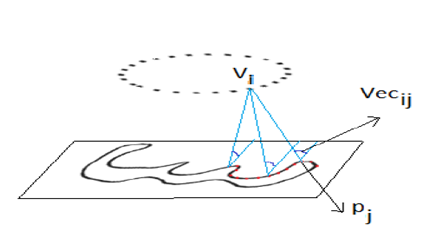
\includegraphics{./figures/mad_demo}       
\caption{In this figure we can see an example of three line segments drawn from the same viewpoint $V_i$, generating the three angles $Vec_{ij}$ with the plane of the shape. When the parameter $j$ goes over all contour points we get the vector $Vec_i$ describing the shape from the view point $V_i$ with the parameter $i$ goes over all viewpoints.}
\label{fig:mad_demo}
\end{figure}

\newpage{}

\section{Metric Embedding}
Given two distributions, it is important to define a quantitative measure of their dissimilarity, with the intent of approximating perceptual dissimilarity as well as possible. Defining a distance between two distributions requires first a notion of distance between the basic features that are aggregated into the distributions. This is known as \emph{ground distance}.
Mathematically, it would be convenient if these distribution distances were true metrics, which would lead to more efficient data structures and search algorithms. As well, this characteristic is usually required in important kernel based classification techniques. For example, to be able to run efficiently "Radial basis function" (RBF) one needs to calculate efficiently the distance between two samples. The dissimilarity metric that we have used is the Earth Movers Distance (EMD). EMD has experimentally verified to capture well the perceptual notion of a difference between images. Piotr Indyk has suggested an embedding technique in which the un-normed EMD metric is embedded into a normed space, so that the distance between the two images is comparable to the distance between the two points which represent the embedding of the two images.

\emph{[EMD approximation. Do we approximate the EMD and then do the embedding? Or we do the embedding within the EMD calculation?]}

\subsection{Earth Movers Distance}
Earth movers distance (EMD) is a measure of the dissimilarity between two histograms. Descriptively, if the histograms are interpreted as two different ways of piling up a certain amount of dirt, the EMD is the minimal cost of turning one pile to other, where the cost is assumed to be the amount of dirt moved times the distance by which it moved.
EMD has been experimentally verified to capture well the perceptual notion of a difference between images \cite{indyk2003fast}.  Computing EMD is based on a solution to the well-known transportation problem. It can be computed as the minimal value of a linear program. 
\emph{[EMD formal definition]}
EMD naturally extends the notion of a distance between single elements to that of a distance between sets, or distributions, of elements when used to compare distributions with the same overall mass, the EMD is a true metric. The major hurdle to using EMD is its $O\left( {{N^3}\log N} \right)$ computational complexity (for an N-bin histogram).Various approximation algorithms have been proposed to speed up the computation of EMD. 
The embedding of EMD given in \cite{indyk2003fast} provides a way to map weighted point sets A and B from the metric space into the normed space $L_1$, such that the $L_1$ distance between the resulting embedded vectors is comparable to the EMD distance between A and B. The motivation of doing so is that the working with normed space is desirable to enable fast approximate Nearest Neighbors (NN) search techniques such as LSH and kdTree. A work conducted by Shirdhonkar and Jacobs in \cite{shirdhonkar2008approximate} has proposed a method for approximating the EMD between two low dimensional histograms using a new on the weighted wavelet coefficients of the difference histogram. The approximation is done by transforming the histograms to $L_1$ space so that the distance between the two vectors in the wavelet domain is the EMD approximation. They have proven the ratio of EMD to wavelet EMD is bounded by constants. The wavelet EMD metric can be computed in $O\left( N \right)$ time complexity.


\subsection{Approximate Earth Movers Distance Embedding}

\subsection{Clustering}
\begin{itemize}
\item Talk about the clustering process.
\item try to implement the number of clusters recommendation system.
\subsubsection{L1 K-medoids}
\end{itemize}

\section{Features Transformation and Dimensionality Reduction}

Answer the following:
\begin{itemize}
\item what is DR and what is its important properties?
\item why do we need DR?
\item what type of DR are there - kernel based, bla bla bla?
\item why did we have choosen to use this DR although we are working in $L_1$ and PCA and LDA word in $L_2$?
\item what package we had used to try different DR techniques?
\item why did we combine LDA and PCA?
\end{itemize}

{\color{blue}When performing analysis of complex data one of the major problems stems from the number of variables involved. Analysis with a large number of variables generally requires a large amount of memory and computation power or a classification algorithm which overfits the training sample and generalizes poorly to new samples. Feature extraction is a general term for methods of constructing combinations of the variables to get around these problems while still describing the data with sufficient accuracy. (Word base line detection in handwritten text recognition systems -- Kamil R. Aida-zade and Jamaladdin Z. Hasanov)}

Feature transformation is a group of methods that create new features (predictor variables). The methods are useful for dimension reduction when the transformed features have a descriptive power that is more easily ordered than the original features. There are 2 main approaches for this task. One is \emph{feature selection} and the other is \emph{feature transformation}. 

Dimensionality Reduction is a process of reducing the number of random variables taken into consideration in the learning and classification of Data. Ideally, the reduced representation should have a dimensionality that corresponds to the intrinsic dimensionality of the data. Reducing the dimensionality of the features vectors would not only simplify and rapid the learning and classification task but rather boosts the classification accuracy.  Feature transformation technique is much more suitable to be implemented in our approach. In this work we have chosen to use two techniques applied in sequential manner in order to obtain the most efficient and linearly discriminative components, \emph{Principle Component Analysis} (PCA) and \emph{Linear Discrimination Analysis} (LDA) Technique. 

\subsection{Principle Component Analysis}
PCA was invented in 1901 by Karl Pearson. It is a linear technique for dimensionality reduction, which means that it performs dimensionality reduction by embedding the data into a linear subspace of lower dimensionality. Although there exist various techniques to do so, PCA is by far the most popular (unsupervised) linear technique. PCA is an orthogonal linear transformation that transforms the data to a new coordinate system such that the greatest variance by any projection of the data comes to lie on the first coordinate (names the first principal component), the second greatest variance on the second coordinate, and so on. Each principal component is a linear combination of the original variables. All the principal components are orthogonal to each other, so there is no redundant information. The principal components as a whole form an orthogonal basis for the space of the data.
The full set of principal components is as large as the original set of variables. But taking the first few principal components will preserve most of the information in the data, and reduces the data dimensions.

\subsection{Linear Discriminant Analysis}
PCA is an unsupervised technique and as such does not include label information of the data. The following example demonstrates the problem drawback: Imagine 2 cigar like clusters in 2 dimensions, one cigar has $y = 1$ and the other $y = -1$. The cigars are positioned in parallel and very closely together, such that the variance in the total data-set, ignoring the labels, is in the direction of the cigars. For classification, this would be a terrible projection, because all labels get evenly mixed and we destroy the useful information. A much more useful projection is orthogonal to the cigars, i.e. in the direction of least overall variance, which would perfectly separate the data-cases.

LDA is closely related to PCA in that they both look for linear combination of variables which best explain the data. LDA explicitly attempts to model the difference between the classes of data. In this method, variability among the feature vectors of the same class is minimized and the variability among the feature vectors of different classes is maximized.

The LDA performs dimensionality reduction while preserving as much of the class discriminatory information as possible. Without going into the math, in order to find a good projection vector, we need to define a measure of separation between the projections. The solution proposed by Fisher is to maximize a function that represents the difference between the means, normalized by a measure of the within-class scatter.

Although, LDA assumes that the distribution of samples in each class is Gaussian and that we cannot prove that the handwritten letters are distributes in a Gaussian manner, we selected LDA as 

Even though LDA is preferred in many application of dimension reduction, it does not always outperform PCA. In order to optimize discrimination performance in a more generative way, a hybrid dimension reduction model combining PCA and LDA is used in this work. 

\subsection{Implementation Details and Discussion}

In this system, we use a flavor the dimensionality reduction process can be outlines as follows: the pre-processed feature matrix $M$ projected into subspace $S_1$ using PCA and then into the subspace $S2$ using LDA. In the PCA stage, the largest $t$ eigenvalues are selected to create the PCA projection matrix $W_{PCA}$. $t$ is the number of eigenvalues which guarantee energy E is greater than 0.99. The data preservation value is calculates as seen in Equation \ref{eq:dr_energy} where ${\lambda _i}$ is the ith eigenvalue

\begin{equation}
E = {{\sum\limits_{i = 1}^t {{\lambda _i}} } \mathord{\left/
 {\vphantom {{\sum\limits_{i = 1}^t {{\lambda _i}} } {\sum\limits_{i = 1}^{\dim \left( S \right)} {{\lambda _i}} }}} \right.
 \kern-\nulldelimiterspace} {\sum\limits_{i = 1}^{\dim \left( S \right)} {{\lambda _i}} }}
\label{eq:dr_energy}
\end{equation}

The dimensionality of $W_{PCA}$ is much smaller that the dimensionality of $M$. At the second phase LDA is used to project $W_{PCA}$ to $W_{PCA+LDA}$.  The dimension of subspace $S_2$ is smaller than the subspace $S_1$ by 1.
Why we have used both and what give us every method and how we did join them together to get the most out of both.

\emph{Why we have used both and what give us every method and how we did join them together to get the most out of both.}

\emph{ Talk about other Dimensionality reduction techniques such as LMNN and show results.}


\section{Letters Classification and Scoring}

In our framework, sub-strokes classification is done by finding a stored letter sample that is maximally similar to the shape of the sub-stroke.

For a given sub-stroke, we need to find the most perceptually close object in the sample set. Since our samples space is in $L_1$ we use NN classification method.

Mention that sub-stroke passes all the processes of preprocessing, feature extraction and classification, embedding, and then using kdtree the list of $N$ objects in the sample set is retrieved. [beware of the dimensionality reduction.]
For each candidate a scoring is given to simulate the extend of resemblance between the sub-stroke and each sample. The scoring is based on the manhattan distance between the sample and the substroke and the Restricted DTW.   

{\color{blue}To reduce the search space,we apply a series of filters in a hierarchicalmanner. The earlier filters perform light processing on a large number of candi- dates, and the later filters perform heavy processing on a small number of candidates. In the first filter, global fea- tures and delayed strokes patterns are used to reduce can- didate word-part models. In the second filter, local features are used to guide a dynamic time warping (DTW) classifi- cation. The resulting k top ranked candidates are sent for shape-context based classifier, which determines the recog- nized word-part. In this work, we have modified the classic DTW to enable different costs for the different operations and control their behavior\cite{saabni2009hierarchical}}

\subsection{Kd-tree}

Example of how to write:
{\color{blue}One of the simplest classifiers we can use is the Nearest Neighbour classifier. This takes a test point in vector form, and finds the Euclidean distance between this and the vector representation of each training example. The training example closest to the test point is termed its Nearest Neighbour. Since this example is in some sense the one most similar to our test point, it makes sense to allocate its class label to the test point. This exploits the 'smoothness' assumption that points near each other are likely to have the same class.}

\subsection{Data Time Warping}

Answer the following:
\begin{itemize}
\item How is the classification is done - mention that the system recieves a stroke and it goes over all the stages
\item A list of candidates is retrieved by the kdtree, then to be more precise we use a combination of the Constrained DTW metric and the distance of the sample and the candidate.
\item mention the alternatives - using different combination (we can afford using heavy tools since we have small candidate number)
\item we return the best 3 candidates.
\end{itemize}

\subsection{Implementation Details and Discussion}
 
\end{document}
